\documentclass[
  accentcolor=tud1c,	% Color theme for TUD corporate design
  colorbacktitle,		% Titlepage has colored background for title area
  inverttitle,			% Font color of title on titlepage is inverted
  german,				% Document is in english
  twoside
]{tudexercise}

\usepackage[ngerman]{babel}
\usepackage{units}
\usepackage{hyperref}
\usepackage[utf8]{inputenc}
\usepackage{algorithm2e}

\definecolor{commentgreen}{RGB}{50,127,50}


\usepackage{listings}
\usepackage{listings}
\lstloadlanguages{C++}
\lstset{language=C++}
\lstset{captionpos=b}
\lstset{tabsize=3}
\lstset{breaklines=true}
\lstset{columns=flexible,keywordstyle=\color{purple},stringstyle=\color{blue},commentstyle=\color{commentgreen}}
\lstset{literate=%
{Ö}{{\"O}}1
{Ä}{{\"A}}1
{Ü}{{\"U}}1
{ß}{{\ss}}2
{ü}{{\"u}}1
{ä}{{\"a}}1
{ö}{{\"o}}1
{'}{{\textquotesingle}}1
}

\parindent0pt

\newcommand{\tag}{1}

\title{Übung zum\linebreak[1]C/C++-Praktikum\linebreak[1] Fachgebiet Echtzeitsysteme}
\subtitle{Übungen für den \tag{}. Tag}

\begin{document}

\begin{examheader}
	\textmb{Übung zum C/C++-Praktikum - Tag \tag{}}
\end{examheader}
\maketitle 

\vspace{5mm}

\section{Eclipse CDT}

Für alle Übungen des C/C++ Praktikums werden wir Eclipse zusammen mit dem C/C++ Development Tooling (CDT) und dem MinGW gcc Compiler verwenden. Es wird davon ausgegangen, dass Sie den generellen Umgang Eclipse bereits aus der Java-Programmierung kennen und nur die Unterschiede zur C++-Programmierung erläutert werden müssen. \\ 

Alle Tools sind bereits auf den Poolrechnern vorinstalliert. Falls Sie mit ihrem Nodebook arbeiten möchten, können Sie den Installer von \href{http://130.83.199.65/download/cplusplus/Eclipse-CPPP.exe}{http://130.83.199.65/download/cplusplus/Eclipse-CPPP.exe} beziehen.\\

Verwenden Sie zum Starten von Eclipse den \textbf{Eclipse für CPPP $\rightarrow$ Eclipse} Eintrag im Startmenü bzw. das \textbf{eclipse.cmd} Script im Installationsordner. Starten Sie \emph{eclipse.exe} nicht direkt, weil dann nicht alle benötigten Pfade gesetzt werden. 

\subsection{Toolchain einstellen}

Als erstes muss MinGW als die bevorzugte C/C++ Toolchain eingestellt werden. Öffnen Sie dazu den Menüpunkt \textbf{Window $\rightarrow$   Preferences} und wählen Sie \textbf{C/C++ $\rightarrow$  New CDT project wizard}. Markieren Sie nun \textbf{MinGW GCC} rechts in der Liste und klicken Sie auf \textbf{Make toolchain(s) preferred}. Schließen Sie den Dialog anschließend mit \textbf{OK}.\\

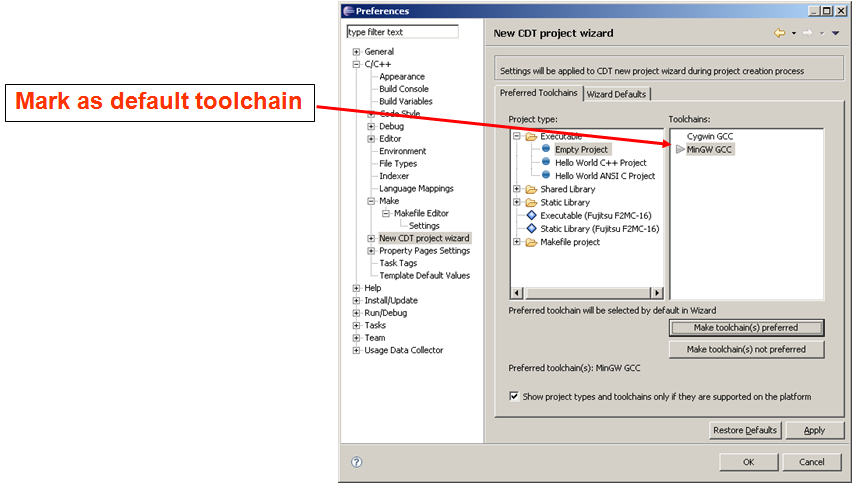
\includegraphics[width=1\textwidth]{toolchain.png}

\subsection{Neues Projekt anlegen}
Um ein neues Projekt anzulegen, wählen Sie \textbf{File $\rightarrow$ New $\rightarrow$ C++ Project} im Eclipse Menü. Geben Sie den gewünschten Projektnamen ein und wählen Sie \textbf{Empty Project} bzw. \textbf{Hello World C++ Project} als Projekttyp aus. Die Toolchain sollte bereits automatisch auf MinGW voreingestellt sein.\\

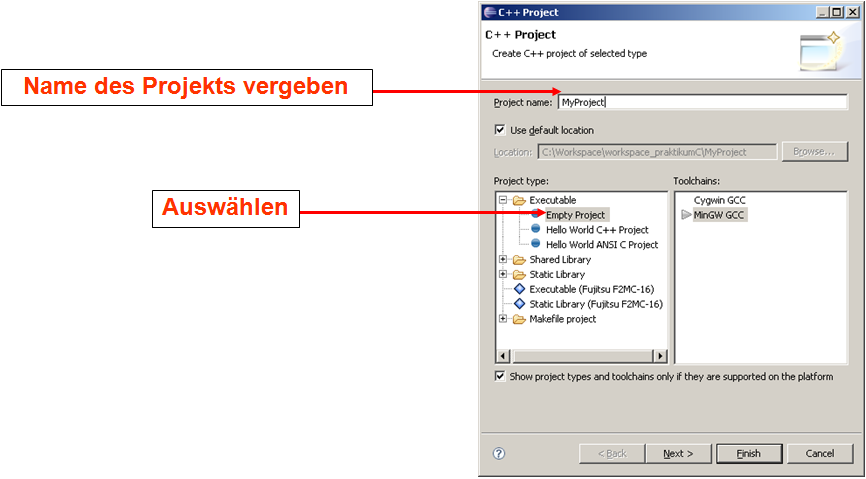
\includegraphics[width=1\textwidth]{new_project.png}

\subsection{Neue Dateien hinzufügen}

Um eine neue Sourcecode-Datei zum Projekt hinzuzufügen, klicken Sie mit der rechten Maustaste auf das Projekt und wählen Sie \textbf{New $\rightarrow$ Source File}. Geben Sie einen Dateinahmen ein und bestätigen Sie mit 
\textbf{Finish}. Verfahren Sie analog, um Header-Dateien zu erstellen, wählen Sie jedoch \textbf{New $\rightarrow$ Header File} im Kontextmenü. Sourcecode-Dateien tragen in der Regel die Endung \emph{.cpp}, Header-Dateien \emph{.h}, \emph{.hpp} oder gar keine Endung. Wir empfehlen Ihnen jedoch \emph{.h} zu benutzen. \\

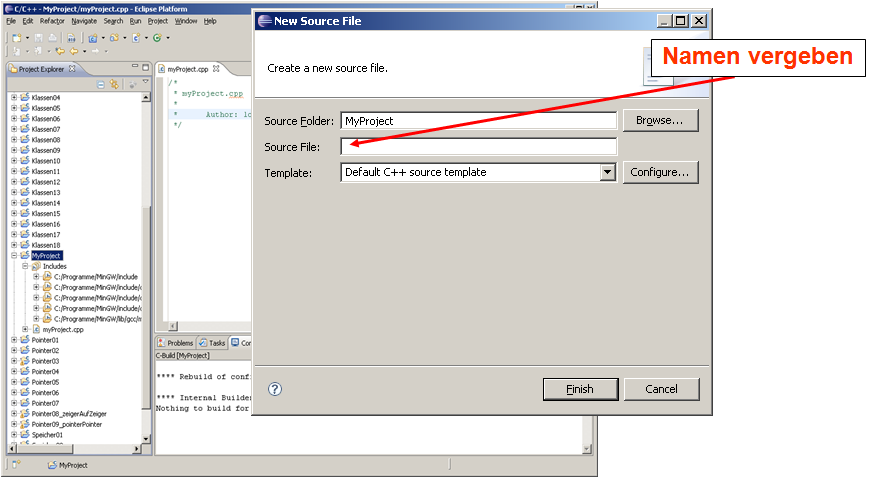
\includegraphics[width=1\textwidth]{new_file.png}

\subsection{Neue Klassen hinzufügen}

Für eine Klasse kann man sowohl den Header als auch die Sourcecode-Datei in einem Schritt erzeugen. Wählen Sie dazu \textbf{New $\rightarrow$ Class} im Kontext-Menü des Projekts, um den Wizard zu starten. Geben Sie den Namen und bei Bedarf den Namespace sowie weitere Informationen wie z.B. die Elternklassen ein (dazu später mehr). Setzen Sie für die ersten Aufgaben den \textbf{virtual} Modifier des Destruktors auf \textbf{No}.

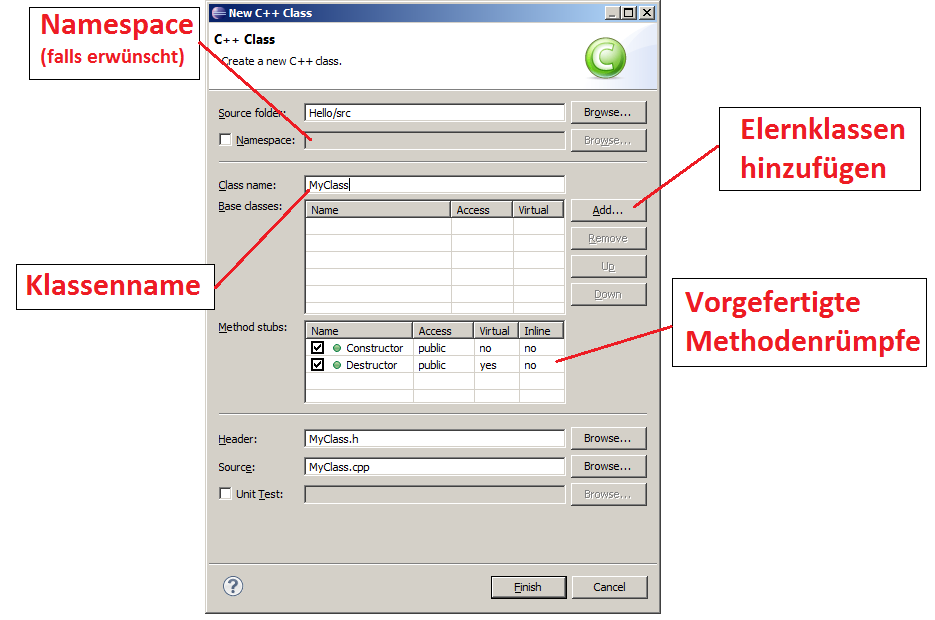
\includegraphics[width=1\textwidth]{class_wizard.png}

\subsection{Projekt kompilieren und starten}

Bevor ein C++-Programm gestartet werden kann, muss es compiliert werden. Im Gegensatz zu Java wird der Compiler nicht automatisch von Eclipse im Hintergrund aufgerufen, sondern muss manuell gestartet werden. Um das aktuell offene Projekt zu kompilieren, klicken Sie auf das \textbf{Build-}Symbol in der Eclipse C++ Toolbar. Im \textbf{Console-}Fenster unten werden Compiler-Meldungen und eventuelle Fehler während des Erstellungsprozesses angezeigt. \\

Um ein kompiliertes Projekt zum ersten mal zu starten, öffnen Sie mit der rechten Maustaste das Kontextmenü des Projekts und wählen Sie \textbf{Run As$\rightarrow$ Local C/C++ Application }.
Danach können Sie zum Starten den grünen Run-Knopf benutzen. \\

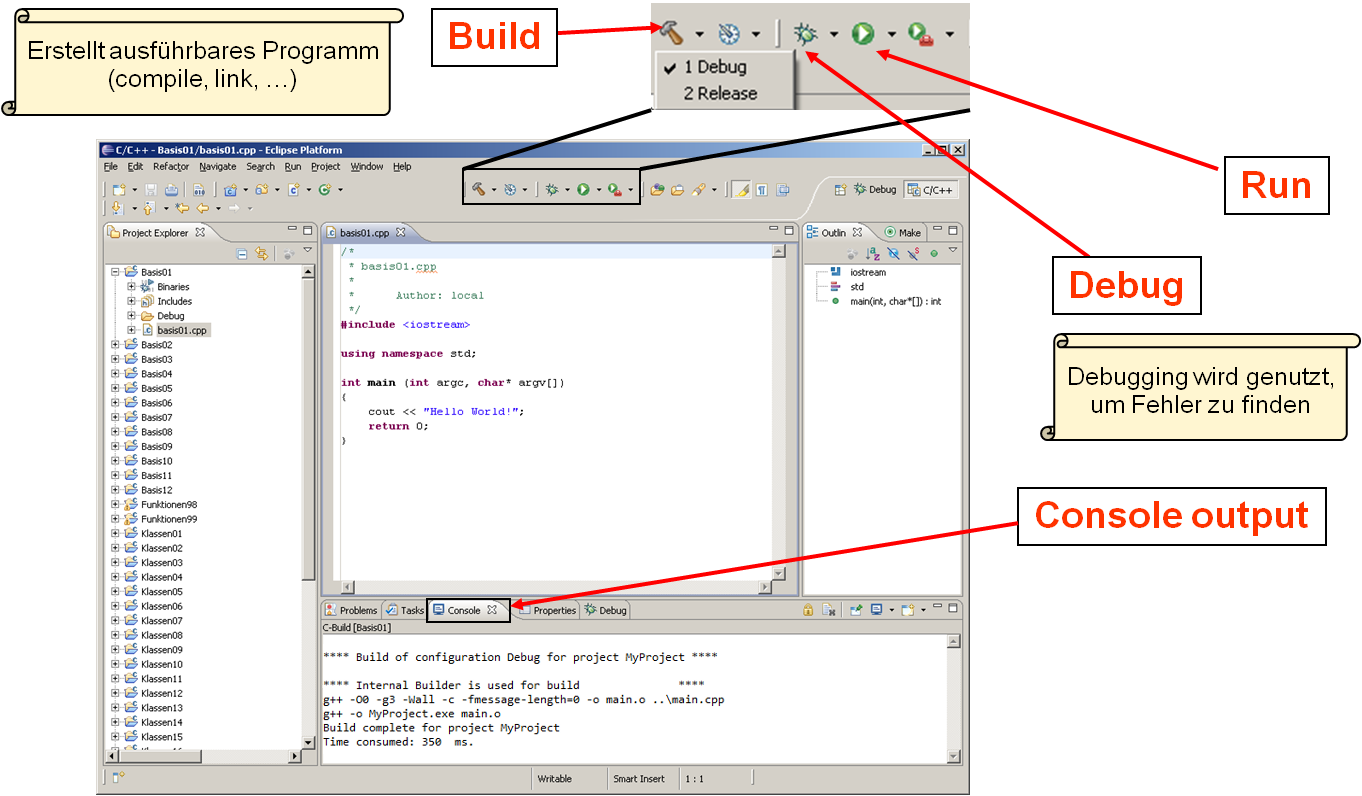
\includegraphics[width=1\textwidth]{build_run.png}

\subsection{Projekt debuggen}
Falls sich im Projekt Fehler einschleichen, die nicht durch einfaches Hingucken behoben werden können, kann es sinnvoll sein, ein Projekt zu debuggen, also die Anweisungen Schritt für Schritt die durchzugehen und die aktuellen Variablen anzuschauen. Dazu muss das Projekt durch drücken des Debug-Knopfes im Debug-Modus gestartet werden. Zum Debuggen wird Eclipse automatisch in die Debug-Perspektive wechseln. \\

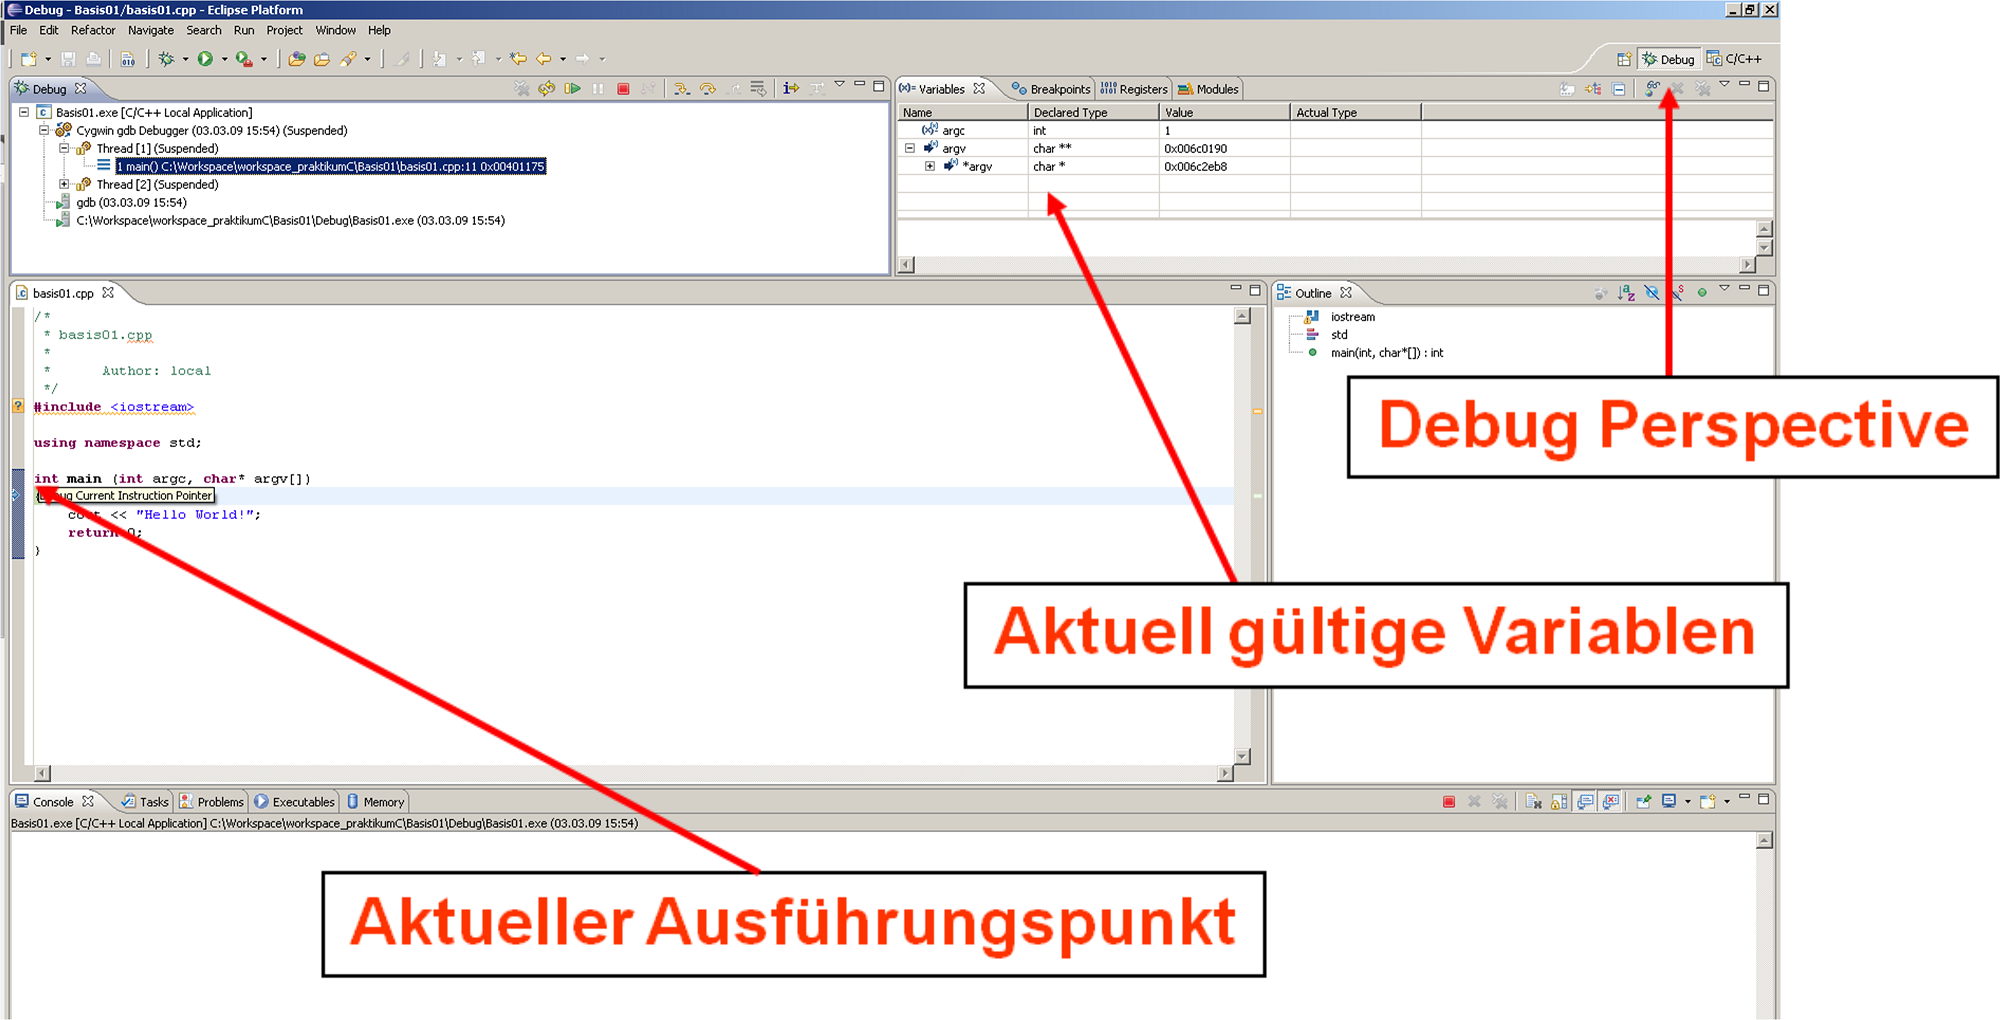
\includegraphics[width=1\textwidth]{debug.png}

\subsection{Erklärung des Hello-World Projekts}
Wenn Sie \textit{Hello World C++ Project} als Projekttyp ausgewählt haben, wird der Wizard automatisch ein Beispiel-Projekt erzeugen, welches \textbf{!!!Hello World!!!} auf der Konsole ausgibt. Wir werden den generierten Code nun stückweise durchgehen und näher erklären.  \\

\begin{lstlisting}
	#include <iostream>
\end{lstlisting}

Die erste Zeile bindet den Header \emph{iostream} ein. Dieser
enthält unter anderem Klassen und Funktionen zur Ein- und Ausgabe. Beachten Sie, dass es zwei verschiedene Möglichkeiten gibt, eine Header-Datei einzubinden -  per \textbf{\#include <...>} sowie per \textbf{\#include "..."}. Bei der ersten Variante sucht der Compiler nur in den Include-Verzeichnissen der Compiler-Toolchain, während bei der zweiten Variante auch die Projektordner durchsucht werden. Somit eignet sich die erste Schreibweise für System-Header und die zweite für eigene, projektspezifische Header. \\

\begin{lstlisting}
	using namespace std;
\end{lstlisting}
Die zweite Zeile bewirkt, dass der namespace \emph{std} eingebunden wird. Ähnlich wie Package-Namen in Java, dienen Namespaces (Namensräume) in C++ zur Strukturierung des Codes und zur Gruppierung von Elementen wie Funktionen und Klassen. Durch Namespaces können Namenskonflikte innerhalb von verschiedenen Bibliotheken vermieden werden. Anders als in Java sind Namespaces in C++ eher kurz und nur sehr selten verschachtelt.\\

Der Namespace der C++Standardbibliothek \emph{Standard Template Library (STL)} ist \emph{std}. Um ein Element aus der  
\emph{STL} zu verwenden, müsste man vor jedem Aufruf ein \emph{std::} setzten, z.B. \emph{std::cout} um Ausgaben auf der Konsole zu tätigen. Durch die Einbindung des kompletten Namespaces mittels \textbf{using namespace std;} ist dies nicht mehr nötig. Bei Bedarf können auch einzelne Elemente des Namespaces eingebunden werden, z.B. durch \textbf{using std::cout;} 

\begin{lstlisting}
	int main() {
		...
	}
\end{lstlisting}

Die Main-Funktion stellt den Einstiegspunkt des Programms dar. Anders als in Java können Funktionen auch außerhalb von Klassen definiert und verwendet werden. Durch die Rückgabe eines \emph{int}s kann das Programm ihrem Aufrufer, also dem Betriebssystem oder der Shell, Erfolg oder Misserfolg der Ausführung mitteilen. Typischerweise signalisieren 0 Erfolg und Werte kleiner 0 einen Fehler. Auf das Programm selbst hat der Rückgabewert keinen Einfluss. \\

Jedes vollständige C++ Programm muss eine \emph{main()}-Funktion besitzen. Andernfalls wird der Linker mit der Fehlermeldung \textbf{undefined reference to 'main'} abbrechen.\\

\begin{lstlisting}
	cout << "!!!Hello World!!!" << endl; // prints !!!Hello World!!!
\end{lstlisting}
Durch \textbf{cout $<<$ ... $<<$ ...} können verschiedene Werte auf der Konsole ausgegeben werden. Ein \textbf{endl} beendet die aktuelle Zeile mit einem Zeilenvorschub. \textbf{//} leitet einen einzeiligen Kommentar ein. Mehrzeilige Kommentare werden in \textbf{/* ... */} eingeschlossen.

\subsection{Häufige Compiler-Fehlermeldungen des gcc}

\begin{verbatim}
error: expected ';' before ...
\end{verbatim}

Dies bedeutet, dass in der Zeile davor ein \textbf{;} vergessen wurde. Allgemein beziehen sich Fehlermeldungen \textbf{expected ... before ...} häufig auf die Zeile \textbf{vor} dem markierten Statement. Beachten Sie, dass \emph{die Zeile davor} auch die letzte Zeile einer eingebundenen Header-Datei sein kann. Beispiel:

\begin{lstlisting}
#include "main.h"
int main() {
	...
}
\end{lstlisting}

Falls im Header \emph{main.h} in der letzten Zeile ein Semikolon fehlt, wird der Compiler die Fehlermeldung trotzdem auf die Zeile \textbf{int main() \{} beziehen!!\\

\begin{verbatim}
error: invalid conversion from <A> to <B>.
\end{verbatim}

Dies bedeutet, dass der Compiler an der entsprechenden Stelle einen Ausdruck vom Typ \emph{B} erwartet, im Code jedoch ein Ausdruck vom Typ \emph{A} angegeben wurde. Insbesondere bei verschachtelten Typen sowie (später vorgestellten) Zeigern und Templates kann die Fehlermeldung sehr lang werden. In so einem Fall lohnt es sich, den Ausdruck in mehrere Teilausdrücke aufzubrechen und die Teilergebnisse durch temporäre Variablen weiterzureichen.\\

\begin{verbatim}
undefined reference to ...
\end{verbatim}

Dies bedeutet, dass das Programm zwar korrekt kompiliert wurde, der Linker aber die Definition des entsprechenden Bezeichners nicht finden kann. Das kann passieren, wenn man dem Compiler durch einen Prototypen mitteilt, dass eine bestimmte Funktion existiert, diese aber nirgendwo tatsächlich definiert. Überprüfen Sie in diesem Fall, ob der Bezeichner tatsächlich definiert wurde und ob die Signatur der Definition mit dem Prototypen übereinstimmt. \\

\subsection{Primitive Datentypen}
Die primitiven Datentypen in C++ sind größtenteils identisch zu den aus Java. Allerdings sind alle Ganzzahl-Typen in C++ sowohl mit als auch ohne Vorzeichen verfügbar. Standardmäßig sind Vorzeichen möglich, mittels \textbf{unsigned} kann man aber vorzeichenlose Variablen deklarieren. Dabei wird der Definitionsbereich entsprechend erweitert, da nun ein Bit mehr zur Verfügung steht.

\begin{lstlisting}
 	int i; // signed int, -2147483648 to +2147483647 on 32-bit machine
	unsigned int ui; // unsigned int, 0 to 4294967295 on 32-bit machine
\end{lstlisting}

Eine andere Besonderheit von C++ ist dass Ganzzahlwerte implizit in \emph{bool}-Werte umgewandelt werden. Alles ungleich 0 wird als \textbf{true} gewertet, 0 als \textbf{false}. Somit können Ganzzahlen direkt in Bedingungen ausgewertet werden:

\begin{lstlisting}
 	int n = 5;
 	// loop which runs until n is 0
 	while(n--) { // post-decrement n, i.e. decrement n but return previous value
  		cout << n << endl;
 	}

	output: 4 3 2 1 0
\end{lstlisting}


\section{C++ Grundlagen, Funktionen und Strukturierung}

Als erstes machen wir uns mit der grundlegenden C++-Syntax vertraut. Diese ist in Grundzügen Java sehr ähnlich, insbesondere die Klammerung und die Kontrollstrukturen wie if/for/while sind beinahe identisch. In den folgenden Aufgaben werden die Unterschiede und Gemeinsamkeiten stückweise erläutert. Falls nicht anders angegeben, können Sie davon ausgehen, dass Sie die gleiche Syntax wie in Java benutzen dürfen.

\begin{enumerate}

\item Legen Sie ein neues \glqq{}Hello World\grqq{}-Projekt an (\textit{File} $\rightarrow$ \textit{New} $\rightarrow$ \textit{C++ Project} $\rightarrow$ \textit{Hello World C++ Project}). Versuchen Sie, das Programm zu kompilieren und zu starten.


\item 
Schreiben Sie eine Funktion \emph{print\_star(int n)}, die \emph{n}-mal ein \textbf{*} auf der Konsole ausgibt und mit einem Zeilenvorschub abschließt. Ein Aufruf von \emph{print\_star(5)} sollte also folgende Ausgabe generieren:
\begin{lstlisting}
*****
\end{lstlisting}

Platzieren Sie die Funktion noch vor der \emph{main}, da sie sonst nicht ohne weiteres aufgerufen werden kann. Benutzen Sie die erstellte Funktion \emph{print\_star(int n)}, um eine weitere Funktion zu schreiben, die eine Figur wie unten dargestellt ausgibt. Verwenden Sie hierzu Schleifen, kodieren sie die Ausgabe der einzelnen Zeilen nicht direkt! 
\begin{lstlisting}
*****
****
***
**
*
**
***
****
*****
\end{lstlisting}

\item
Lagern Sie ihr Programm aus Aufgabenteil b) in eine eigene Datei aus. Gehen Sie dazu
folgendermaßen vor: 

Erstellen Sie eine neue Header-Datei \emph{functions.h} und eine neue Sourcecode-Datei \emph{functions.cpp}. 

Binden Sie \emph{functions.h} in beide Sourcecode-Dateien mittels 
einer entsprechenden \textbf{\#include}-Anweisung ein. Vergessen Sie nicht, auch in \emph{functions.cpp} den \emph{std}-Namespace sowie \emph{iostream} einzubinden, falls Sie dort Elemente der Standardbibliothek benutzen möchten. Vermeiden Sie insbesondere bei echten Programmen bitte unbedingt, den Namespace bereits im Header einzubinden! Dadurch würden alle Dateien, die den Header einbinden, den Namespace ebenfalls einbinden, was zu Namenskonflikten und Überraschungen führen kann. Benutzen Sie deshalb den Scope-Operator \textbf{::} im Header-Code.

Schreiben Sie nun in \emph{functions.h} Funktionsprototypen für die beiden Funktionen aus b). Funktionsprototypen dienen dazu, dem Compiler mitzuteilen, dass eine Funktion mit gegebenen Parametern existiert und aufgerufen werden kann, ohne die Implementierung bereitzustellen. Ein Prototyp ist im wesentlichen eine mit \textbf{;} abgeschlossene Signatur der Funktion ohne Funktionsrumpf. Der Prototyp von \emph{print\_star(int n)} lautet dementsprechend \emph{void print\_star(int n);}

Kopieren Sie Ihre beiden Funktionen nach \emph{functions.cpp}. Nun können aus der main.cpp heraus Funktionen aus \emph{functions.cpp} aufrufen werden.

\item Erweitern Sie das in Aufgabenteil c) erstellte Programm um eine Eingabeaufforderung zur Bestimmung der Breite der auszugebenden Figur. Die Breite soll dabei
eine im Programmcode vorgegebene Grenze nicht überschreiten dürfen. Gibt der Benutzer eine zu große Breite ein, wird er darüber informiert und erneut gefragt. Zum Einlesen benutzen Sie \texttt{cin >{}> \textit{variable}}. Erstellen Sie auch für diesen Aufgabenteil eine eigene Funktion und lagern Sie diese nach \emph{functions.cpp} aus.

\item Statt einem einzigen Zeichen soll nun das fortlaufende Alphabet ausgegeben werden. Sobald das Ende des Alphabets erreicht wurde, soll wieder bei \emph{a} begonnen werden. Beispiel:
\begin{lstlisting}
abc
de
f
gh
ijk
\end{lstlisting}

Implementieren Sie dazu eine Funktion \emph{char next\_char()}. Diese soll bei jedem Aufruf das nächste auszugebende Zeichen von Typ \emph{char} zurückgeben, beginnend bei \emph{\textquotesingle a\textquotesingle}. Dazu muss sich \emph{next\_char()} intern das aktuelle Zeichen merken. Dies kann durch die Verwendung von \emph{static}-Variablen erreicht werden. \emph{static}-Variablen sind Variablen, die ihren alten Wert beim Wiedereintritt in die Funktion einnehmen. Ein statische Variable \emph{c} wird mittels 
\begin{lstlisting}
static char c = 'a';
\end{lstlisting}
deklariert. In diesem Fall wird c \textbf{einmalig zu Beginn des Programms} mit 'a' initialisiert und kann später beliebig verändert werden.\\
\end{enumerate} 

\section{Klassen}

In der vorherigen Übung haben wir den Modifier \textbf{static} verwendet, um eine Funktion zu erstellen, welche fortlaufende Zeichen generiert. Diese Methode hat jedoch mehrere Nachteile, unter anderem kann man die Funktion nicht in mehreren Threads gleichzeitig nutzen, da es zur Interferenz bei der Verwendung der statischen Variable kommen könnte. Deshalb werden wir nun eine Klasse schreiben, welche das aktuelle Zeichen als Attribut enthält und durch Methoden ausgelesen und inkrementiert werden kann. Dadurch können mehrere Instanzen der Klasse nebeneinander existieren, ohne die Zeichenausgabe gegenseitig zu stören.

\begin{enumerate}

\item Legen Sie ein neues Projekt an und fügen Sie dem Projekt eine neue leere Klasse \emph{CharGenerator} hinzu. Obwohl Eclipse Klassenrümpfe automatisch generieren kann, wollen wir aus Übungsgründen die Klasse diesmal manuell erstellen. Erzeugen Sie dazu einen Header \emph{CharGenerator.h} und eine Sourcecode-Datei \emph{CharGenerator.cpp}. Binden Sie \emph{CharGenerator.h} in \emph{CharGenerator.cpp} und in \emph{main.cpp} ein.\\

Erstellen Sie nun den Klassenrumpf von \emph{CharGenerator} in der Header-Datei. Die allgemeine Syntax lautet hierbei 

\begin{lstlisting}
class <Name> { // Echter Name ohne <> 
}; // Semikolon am Ende beachten!
\end{lstlisting}

Genauso wie bei Funktionen wird auch bei Methoden von Klassen zwischen Deklaration und Implementierung unterschieden. Die Struktur der Klasse mit allen Attributen und Methodenprototypen wird im Header beschrieben, während die Sourcecode-Datei nur Implementierungen enthält. Da wir noch keine Methoden definiert haben, unsere Sourcecode-Datei  entsprechend leer.

\item
Fügen Sie Ihrer Klasse nun das Attribut \emph{char nextChar} hinzu, in dem das als nächstes auszugebende Zeichen gespeichert wird. Im Gegensatz zu Java  werden in C++ die Access-Modifier \emph{public}/\emph{private}/\emph{protected} nicht bei jeder Methode einzeln sondern blockweise angegeben. Dazu wird der jeweilige Access-Modifier an die gewünschte Stelle in der Klassendeklaration geschrieben und mit einem Doppelpunkt abgeschlossen.  Alle darauffolgenden Deklarationen werden nun unter diesem Modifier erstellt. Beispiel:

\begin{lstlisting}
class Foo { 
public:
	void ichBinPublic(); // public Methode
	... // weitere Methoden/Attribute
protected:
	void ichBinProtected(); // protected Methode
	...
private:
	void ichBinPrivate(); // private Methode
	...
};
\end{lstlisting}

Fügen Sie das Attribut \emph{nextChar} als \textbf{private} hinzu.

\item Noch wurde \emph{nextChar} keinen Wert zugewiesen. Das wollen wir nun nachholen und einen Konstruktor für die Klasse \emph{CharGenerator} erstellen, der \emph{nextChar} auf einen Anfangswert setzt. Der Konstruktor wird als eine Methode ohne Rückgabetyp definiert, die den gleichen Namen wie die Klasse hat, und beliebige Parameter beinhalten kann, in unserem Fall also 
\begin{lstlisting}
CharGenerator();
\end{lstlisting}

Erstellen Sie den Konstruktorprototypen im \emph{public}-Bereich der Klasse und eine Implementierung in der Sourcecode-Datei. Damit der Compiler weiß, zu welcher Klasse eine Methode/Konstruktor gehört, muss man vor dem Methodennamen den Scope der Klasse angeben.

\begin{lstlisting}
CharGenerator::CharGenerator() {  // Konstruktor von CharGenerator.
	...
}
\end{lstlisting}

Um \emph{nextChar} einen Wert zuzuweisen, werden wir eine sogenannte Initialisierungsliste verwenden. Diese beschreibt, welches Attribut mit welchem Wert initialisiert wird, bzw. welcher Konstruktor für die Erzeugung von Objektattributen verwendet werden soll. Dadurch wird garantiert, dass beim Eintritt in den Konstruktorrumpf alle Objektattribute bereits initialisiert sind und verwendet werden dürfen. Die Initialisierungsliste wird durch einen Doppelpunkt zwischen der schließenden Klammer der Parameterliste und der geschweiften Klammer des Rumpfes eingeleitet, und bildet eine mit Komma separierte Liste von Attributennamen und ihren Initialisierungsargumenten in Klammern. Beispiel:

\begin{lstlisting}
CharGenerator::CharGenerator(): nextChar('a') {
}
\end{lstlisting}

Initialisieren Sie nun \emph{nextChar} mit 'a' durch die oben beschriebene Weise.

\item Schreiben Sie nun eine public Methode \emph{char generateNextChar()} die analog zur vorherigen Aufgabe das nächste auszugebende Zeichen zurückgibt. Teilen Sie die Methode in Prototyp und Implementierung auf. Vergessen Sie auch hier nicht, den Scope der Klasse bei der Implementierung anzugeben:

\begin{lstlisting}
char CharGenerator::generateNextChar() {
	...
}
\end{lstlisting}

\item Testen Sie Ihre Implementierung. Legen Sie in der main ein \emph{CharGenerator}-Objekt mittels \textbf{CharGenerator charGen;} an. Ein \textbf{new} ist dabei nicht erforderlich (näheres dazu in der nächsten Vorlesung).

Machen Sie einige Aufrufe von \emph{generateNextChar()} und geben Sie das Ergebnis auf der Konsole aus.

\item Wir wollen nun angeben können, mit welchem Zeichen unser \emph{CharGenerator} beginnen soll. Erweitern Sie dazu den Konstruktor um einen Parameter \emph{char initialChar} und ändern sie die Initialisierung von \emph{nextChar}, damit dieser mit dem übergebenen Parameter gestartet wird.

Damit man nicht immer das Startzeichen angeben muss, kann man sogenannte \emph{Default Parameter} angeben. Weisen Sie hierzu den jeweiligen Parameter im Prototypen einfach einen Wert zu. An der Implementierung muss nichts geändert werden.
\begin{lstlisting}
class CharGenerator {
public:
	CharGenerator(char initialChar = 'a');
	...
};
\end{lstlisting}

Nun ist die Angabe des Startzeichens optional und kann auf Wunsch weggelassen werden. Beachten Sie, dass bei der Definition eines Default-Parameters für alle nachfolgenden Parameter ebenfalls Default-Werte angegeben werden müssen, um Mehrdeutigkeiten beim Aufruf zu vermeiden. 

Testen Sie Ihre Implementierung sowohl mit als auch ohne Angabe des Startzeichens. Um ein Startzeichen anzugeben, legen Sie das Objekt mittels \textbf{CharGenerator charGen('x');} an.

\item Erstellen Sie eine neue Klasse \emph{PatternPrinter} und fügen Sie ein \emph{CharGenerator}-Objekt \emph{charGenerator} als privates Attribut hinzu. Erstellen Sie auch einen leeren, parameterlosen Konstruktor.

Ohne eine Initialisierungsliste wird \emph{charGenerator} mit dem default-Parameter initialisiert. Um ein eigenes Startzeichen anzugeben, muss eine Initialisierungsliste erstellt und \emph{charGenerator} mit dem entsprechenden Argument initialisiert werden.

\item Erstellen Sie die Methoden \emph{void printNChars(int n)}, \emph{int readWidth()} und \emph{void printPattern()}, die entsprechend n Zeichen auf die Konsole ausgeben, die Breite einlesen und unter Verwendungen aller Methoden das Muster aus der vorherigen Aufgabe auf der Konsole ausgeben. \emph{printNChars} sollte hierbei \emph{charGenerator} benutzen, um das nächste Zeichen ermitteln.

Testen Sie Ihre Implementierung, indem Sie ein \emph{PatternPrinter}-Objekt anlegen und \emph{printPattern()} darauf aufrufen.

\end{enumerate}

\section{Operatorüberladung} 
In C++ besteht die Möglichkeit, Operatoren wie \textbf{+}, \textbf{*}, ... in Zusammenhang mit eigenen Klassen zu überladen. Das bedeutet man kann selbst spezifizieren, was beim Verknüpfen von Objekten mit einem Operator geschehen soll, um zum Beispiel den Quellcode übersichtlicher zu gestalten. Sie haben bereits das Objekt \emph{cout} der Klasse \emph{ostream} kennen gelernt, welche den $<<$-Operator überladen hat, um Ausgaben komfortabel zu tätigen. In dieser Aufgabe wollen wir eine eigene Vektor-Klasse schreiben und einige Operatoren überladen.\\

Wir werden am Tag 4 auf dieser Aufgabe aufbauen und den Vektor um weitere Funktionen erweitern. Behalten Sie dies bitte im Hinterkopf und löschen Sie Ihre Lösung nicht. Falls Sie mit dieser Aufgabe bis dahin nicht fertig sein sollten, können Sie natürlich auch die Musterlösung als Basis nehmen.

\begin{enumerate}
\item 
Schreiben Sie eine Klasse \emph{Vector3} mit den Attributen \emph{a}, \emph{b} und \emph{c} vom Typ \emph{double}, die die einzelnen Komponenten eines 3-dimensionalen Vektors darstellt. Die Klasse soll drei Konstruktoren besitzen, einen parameterlosen Default-Konstruktor, der den Vektor mit \textbf{0} initialisiert, einen Konstruktor mit 3 Parametern, der die einzelnen Vektor-Komponenten auf den gegebenen Wert setzt, und einen Copy-Konstruktor. Der Copy-Konstruktor wird aufgerufen, wenn das Objekt kopiert werden soll, z.B. für eine Call-By-Value Parameterübergabe. Er nimmt eine Objekt vom gleichen Typ wie die Klasse selbst (in unserem Fall \emph{Vector3}) als Parameter und kopiert alle Attribute. Die Übergabe sollte dabei per const Reference geschehen. Näheres dazu erfahren Sie morgen. Bis dahin übernehmen Sie einfach die folgende Syntax für den Prototypen:
\begin{lstlisting}
Vector3(const Vector3& other);
\end{lstlisting} 

Sie können \emph{other} wie ein gewöhnliches \emph{Vector3}-Objekt verwenden, es jedoch nicht verändern. \\

Erstellen Sie außerdem einen Destruktor. Ein Destruktor ist eine Methode, die automatisch beim Löschen des Objektes aufgerufen wird. Die Syntax des Prototypen lautet
\begin{lstlisting}
	~Vector3();
\end{lstlisting} 

und die Implementierung entsprechend
\begin{lstlisting}
Vector3::~Vector3() {
	...
}
\end{lstlisting} 

Fügen Sie in beide Konstruktoren und den Destruktor eine Ausgabe auf die Konsole hinzu, um beim Programmlauf den Lebenszyklus der Objekte besser nachvollziehen zu können

\item
Überladen Sie den Operator \textbf{+} der Klasse \emph{Vector3}, der eine komponentenweise Vektoraddition durchführt. Die Signatur lautet
\begin{lstlisting}
Vector3 operator+(Vector3 rhs);
\end{lstlisting}
Das \emph{Vector3} links ist dabei der Rückgabetyp der Überladung, der Parameter rhs die rechte Seite ("{}right-hand-side"{}) des \textbf{+}-Operators. Das eigene Objekt nimmt hierbei automatisch die linke Seite der Operation an. Platzieren Sie den Prototyp im \emph{public}-Bereich der \emph{Vector3} Klasse.

Die Implementierung lautet dementsprechend
\begin{lstlisting}
Vector3 Vector3::operator+(Vector3 rhs) {
	...
}
\end{lstlisting}

Sie können nun innerhalb der Methode durch \emph{a}, \emph{b} und \emph{c} auf eigene Attribute und über  \emph{rhs.a}, \emph{rhs.b} und \emph{rhs.c} auf Attribute der rechten Seite zugreifen.

\item
Überladen Sie auf die gleiche Weise auch die Operatoren $-$ für eine komponentenweise Vektorsubtraktion sowie \textbf{*} für ein Skalarprodukt. Beachten Sie, dass der Rückgabetyp eines Skalarprodukts kein \emph{Vector3} sondern ein Skalar (\emph{double}) ist!

Jetzt können Sie Vektoren durch \emph{v1 + v2}, \emph{v1 - v2} und \emph{v1 * v2} addieren/subtrahieren und das Skalarprodukt bilden.

\item
Um die Korrektheit unserer Implementierung zu testen, brauchen wie eine Ausgabemöglichkeit eines \emph{Vektor3}-Objektes, idealerweise mit der gewohnten \emph{cout \textbf{$<<$} ...} Syntax. Dazu werden wir den \textbf{$<<$} Operator überladen.

Diesmal müssen wir die Überladung \textbf{außerhalb} der \emph{Vektor3}-Klasse definieren, weil auf unser \emph{Vektor3}-Objekt nun auf der rechten Seite der Operation stehen muss. Der Funktionsprototyp lautet 
\begin{lstlisting}
std::ostream& operator<<(std::ostream& out, Vector3 rhs);
\end{lstlisting}

Als linke Seite wird hierbei ein \emph{ostream}-Objekt (wie z.B. \emph{cout}) erwartet. Um Ausgabeketten \emph{cout} \textbf{$<<$} ... \textbf{$<<$} ... zu ermöglichen, muss das Ausgabeobjekt auch zurückgegeben werden. Damit das \emph{ostream}-Objekt nicht jedes Mal kopiert wird, wird es als Referenz \textbf{\&} übergeben.

Zusammengefasst hat die Implementierung folgende Form:
\begin{lstlisting}
ostream& operator<<(ostream& out, Vector3 rhs)  {
	out << ... ;
	return out;
}
\end{lstlisting}

Füllen Sie die Funktion aus und versuchen Sie, das Projekt zu kompilieren. Vergessen Sie nicht, den \emph{iostream} Header und \emph{std} Namespace einzubinden.

\item
Der Compiler wird mit der Fehlermeldung 
\begin{verbatim}
error: 'double Vector3::a' is private within this context
\end{verbatim}
abbrechen. Dies liegt daran, dass die Attribute \emph{a}, \emph{b} und \emph{c} privat und nur innerhalb der Klasse griffbereit sind. Erstellen Sie deshalb Getter-Methoden für die einzelnen Vektorkomponenten und verwenden Sie diese in der Ausgabefunktion. Wenn alles funktioniert hat, können Sie beliebige \emph{Vector3}-Objekte über 
\begin{lstlisting}
cout << v << endl;
\end{lstlisting} 
ausgeben.

\item
Testen Sie ihre bisher definierten Methoden und Funktionen. Probieren Sie auch Kombinationen von verschiedenen Operatoren aus und beobachten Sie das Ergebnis. Schreiben Sie auch eine einfache Funktion, die Vektoren als Parameter nimmt. Wie Sie sehen können, werden sehr viele \emph{Vector3}-Objekte erstellt, kopiert und gelöscht. Dies liegt daran, dass die Objekte immer per Call-By-Value übergeben und dabei kopiert werden. Wie es vermieden werden kann, erfahren Sie im nächsten Teil des Praktikums.

\end{enumerate}

\section{Aufzug}
In dieser Aufgabe soll ein Grundgerüst für den in der Vorlesung vorgestellten Aufzug-Simulator geschaffen werden. Folgendes Klassendiagramm sollte die Klassenstruktur veranschaulichen.

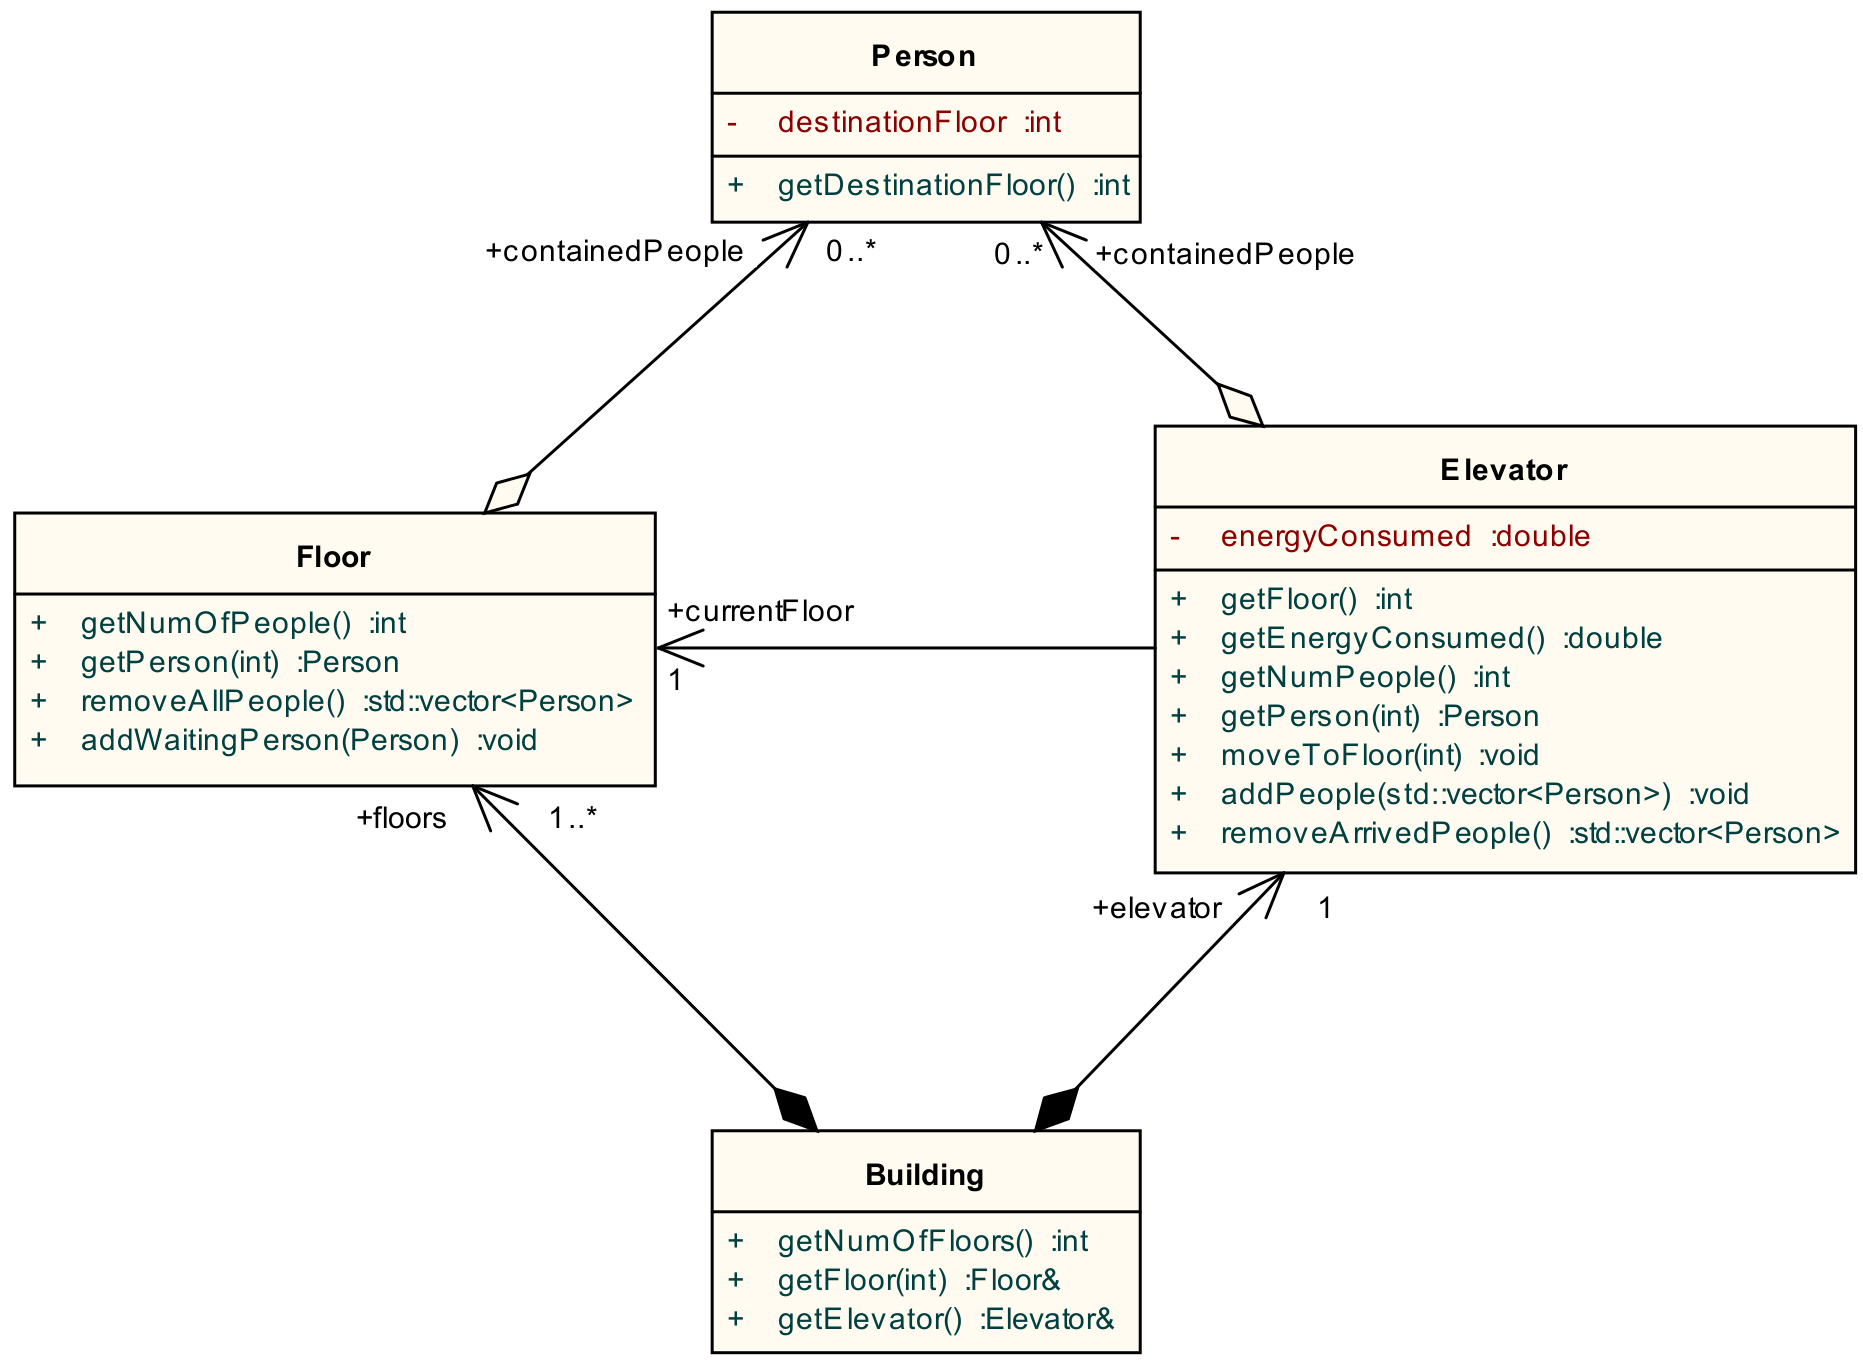
\includegraphics{Aufzug.png}

\begin{enumerate}
\item Schreiben Sie eine Klasse \emph{Person}. Diese soll ein Attribut \emph{int destinationFloor} haben, welches das Zielstockwerk angibt. Initialisieren Sie das Attribut im Konstruktor und schreiben Sie einen entsprechenden Getter. Fügen Sie dem Konstruktor außerdem eine Ausgabe auf die Konsole hinzu, um später beim Programmlauf den Erzeugungsprozess besser nachvollziehen zu können. Erstellen Sie zudem einen Destruktor für \emph{Person} sowie den Copy-Konstruktor. Vergessen Sie nicht, im Copy-Konstruktor \emph{destinationFloor} des anderes Objekts zu übernehmen. Erstellen Sie auch hier eine Konsolenausgabe, um den Lebenszyklus darzustellen.

\item
Schreiben Sie eine Klasse \emph{Elevator} mit den Attributen \emph{int currentFloor}, \emph{double energyConsumed} sowie \emph{std::vector<Person> containedPeople}. Dabei soll \emph{int currentFloor} die Nummer des aktuellen Stockwerks repräsentieren, \emph{double energyConsumed} die verbrauchte Energie. In \emph{containedPeople} werden die sich aktuell im Aufzug befindlichen Menschen gespeichert. Dafür benutzen wir die Klasse \emph{vector} aus dem \emph{std} Namespace. Binden Sie dazu den Header \emph{vector} ein. \emph{vector} ist ein Container, welches ein Array kapselt und eine ähnliche Funktionalität wie Javas \emph{Vector} Klasse bereitstellt. Das \textbf{<Person>} in \emph{std::vector<Person>} ist ein Template-Parameter und besagt, dass in dem Container \emph{Person}-Objekte gespeichert werden sollen. \\

Schreiben Sie Getter für \emph{currentFloor} sowie \emph{energyConsumed}. Implementieren Sie außerdem die Methoden
\begin{lstlisting}
	/** Returns number of people in Elevator */
	int getNumPeople();
	
	/** returns i-th Person in Elevator */
	Person getPerson(int i);
\end{lstlisting} 

Sie können mit \emph{containedPeople.size()} auf die Länge eines vectors zugreifen und mittels \emph{containedPeople.at(i)} auf das i-te Element. \\

Implementieren Sie auch die Methode
\begin{lstlisting}
	/** Moves the elevator to given floor */
	void moveToFloor(int floor);
\end{lstlisting}

die den Aufzug zu einem bestimmten Stockwerk fahren lässt. Passen Sie die verbrauchte Energie entsprechend an, addieren Sie z.B. die Differenz zwischen dem aktuellen und dem Zielstockwerk hinzu.\\

Als letztes müssen wir die Methoden zum Ein- und Aussteigen in/aus dem Aufzug schreiben.
\begin{lstlisting}
	/** add people to Elevator */
	void addPeople(std::vector<Person> people);

	/** remove people which arrived at their destination */
	std::vector<Person> removeArrivedPeople();
\end{lstlisting} 

Sie können dabei \emph{containedPeople.push\_back(Person)} nutzen, um eine einzelne Person 
zur Menge der Insassen hinzuzufügen. Um die Leute aussteigen zu lassen, die an ihrem
  Zielstockwerk angekommen sind, erstellen Sie in der Methode zwei temporäre \emph{vector}-Container
   \emph{stay} und \emph{arrived}. Iterieren Sie nun über alle Leute in dem Aufzug und prüfen Sie, ob das Zielstockwerk der Person mit dem aktuellen Stockwerk des Aufzugs übereinstimmt.
    Wenn ja, lassen Sie die Person aussteigen, indem Sie sie zu der arrived-Liste mittels
     \emph{push\_back()} hinzufügen. Andernfalls muss die Person im Aufzug verbleiben (stay-Liste). 
     Geben Sie am Ende die arrived-Liste zurück, und ersetzen Sie \emph{containedPeople} durch \emph{stay}.

\item Schreiben Sie die Klasse \emph{Floor} mit dem Attribut \emph{std::vector<Person> containedPeople}. Implementieren Sie die Methoden

\begin{lstlisting}
	/** Return number of people on this floor */
	int getNumPeople();
	
	/** return i-th Person on this floor */
	Person getPerson(int i);
	
	/** Add a Person to this floor */
	void addWaitingPerson(Person h);
	
	/** remove all persons from this floor and return them */
	std::vector<Person> removeAllPeople();
\end{lstlisting}

Nutzen Sie \emph{containedPeople.clear()} um alle Elemente eines Vectors zu löschen.

\item
Schreiben Sie eine Klasse \emph{Building}. Der Konstruktor soll dabei die Anzahl der Stockwerke als Parameter erhalten. Fügen Sie einen Aufzug \emph{elevator} sowie \emph{std::vector<Floor> floors} als private Attribute hinzu. Implementieren Sie einen Getter, der den Aufzug als Referenz (\emph{Elevator\&}) zurückgibt. Implementieren Sie dazu die Methoden

\begin{lstlisting}
	/** return number of floors */
	int getNumOfFloors();
	
	/** return a certain floor as reference*/
	Floor& getFloor(int floor);
\end{lstlisting}

analog zur vorherigen Aufgabe.

\item 
Um die Benutzung des Simulators von außen zu vereinfachen und lange Aufrufketten wie
\begin{lstlisting}
	b.getElevator().addPeople(b.getFloor(b.getElevator().getFloor()).removeAllPeople());
\end{lstlisting} 

zu vermeiden, werden wir \emph{Building} einige weitere Methoden hinzufügen. Diese sollen als Zugriffspunkte für den Simulator dienen. Implementieren Sie hierfür folgende Methoden:

\begin{lstlisting}
	/** 
	 * Let people on current floor go into the elevator.
	 */
	void letPeopleIn();
	
	/** remove people from elevator on current floor which arrived at their destination */
	std::vector<Person> removeArrivedPeople();
	
	/** Move the building's elevator to given floor */
	void moveElevatorToFloor(int i);
	
	/** Add a person to given floor */
	void addWaitingPerson(int floor, Person p);
\end{lstlisting}	

\item
Testen Sie Ihre Implementierung. Erstellen Sie dazu zunächst ein Gebäude und fügen Sie einige Personen hinzu.

\begin{lstlisting}
	Building b(3);
	b.addWaitingPerson(0, Person(2)); // person in floor 0 wants to floor 2
	b.addWaitingPerson(1, Person(0)); // person in floor 1 wants to floor 0
	b.addWaitingPerson(2, Person(0)); // person in floor 2 wants to floor 0
\end{lstlisting}

Implementieren Sie nun folgende Beförderungsstrategie. Diese sehr einfache (und ineffiziente) Strategie fährt alle Stockwerke nacheinander ab, sammelt die Leute ein und befördert Sie jeweils zu ihren Zielstockwerken.

\begin{algorithm}[H]
 \SetAlgoLined
 \For{Floor floor \textbf{in} Building}{
   Move Elevator to Floor;\\
   Let all people on Floor into the Elevator;\\
   
  \While{Elevator has people} {
    Move Elevator to destination Floor of first Person in Elevator; \\
    Remove arrived people; \\
  }
 }
\end{algorithm}

Geben Sie am Ende auch die benutze Energie aus. Schauen Sie sich die Ausgabe genau an und versuchen Sie nachzuvollziehen, warum Personen so oft kopiert werden. Denken Sie daran, dass diese bei einer Übergabe als Argument kopiert werden. \\\\

\end{enumerate}

\end{document}
